\documentclass{article}
\usepackage[utf8]{inputenc}
\textheight = 25cm 
\textwidth = 18cm
\topmargin = -3.0cm 
\oddsidemargin = 0.5cm
\usepackage{hyperref}
\hypersetup{
    colorlinks=true,
    linkcolor=blue,
    filecolor=blue,
    citecolor=black,      
    urlcolor=blue,
    }

\usepackage{float}
\usepackage{graphicx}

\usepackage{amsmath}
\usepackage{amssymb}
\usepackage{amsfonts}
\usepackage{mathtools, xparse}
\usepackage[shortlabels]{enumitem}

\usepackage[many]{tcolorbox}
\usepackage{lipsum}

\title{Tarea 5 Matemáticas Avanzadas de la Física}
\author{Cerritos Lira Carlos}
\date{27 de Marzo del 2020}

\begin{document}
\maketitle
\section*{1.-}
En una ciudad se publican tres periódicos, $A,B$ y $C$. Una encuesta reciente muestra que el $20\%$ 
de los habitantes adultos de la ciudad lee el periódico $A$, el $16\%$ lee el periódico $B$, 
el $14\%$ lee el periódico $C$, el $8\%$ lee los periódicos $A$ y $B$, el $5\%$ lee los periódicos $A$ y $C$, 
el $4\%$ lee los periódicos $B$ y $C$, y el $2\%$ lee los tres periódicos. 
Si se sabe que el total de habitantes en la ciudad es de $20,000$ y se elige un adulto al azar,
\begin{enumerate}[a)]
    \item ¿Cuántos habitantes no leen ninguno de los periódicos?
    \item ¿Cuántos habitantes leen exactamente uno de los periódicos?
    \item Si $A$ y $B$ son periódicos que se publican por la mañana y $C$ se publica en la tarde, 
    ¿cuántos habitantes leen al menos un periódico de mañana y uno de tarde?
\end{enumerate}
\begin{tcolorbox}[breakable]
    \subsubsection*{a)}
    \begin{figure}[H]
        \centering
        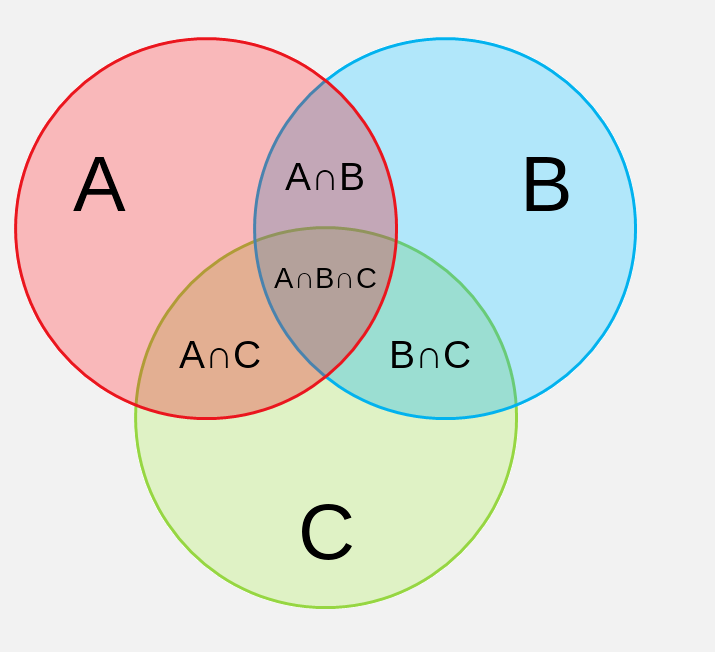
\includegraphics[scale=0.3]{images/p1_venn.png}
        \caption{Diagrama de Venn para los conjuntos $A$,$B$,$C$}
    \end{figure}
    Con ayuda del diagrama de Venn podemos observar:
    \[ P(A \cup B \cup C) = P(\bar{A}) + P(\bar{B}) + P(\bar{C}) + P(A \cap C) + P(A \cap B) + P(B \cap C) - 2P(A \cap B \cap C) \]
    donde $\bar{X}$ son los lectores únicos para el periódico $X$. \\ 
    El número de lectores únicos para cada periódico es:
    \begin{align*}
        P(\bar{A}) 
        &= P(A) - P(A \cap C) - P(A \cap B) + P(A \cap B \cap C) \\
        &= 20 - 5 - 8 + 2 \\
        &= 9 \\
        P(\bar{B}) 
        &= P(B) - P(B \cap C) - P(B \cap A) + P(A \cap B \cap C) \\
        &= 16 - 4 - 8 + 2 \\
        &= 6 \\
        P(\bar{C})
        &= P(C) - P(C \cap B) - P(C \cap A) + P(A \cap B \cap C) \\
        &= 14 - 4 - 5 + 2 \\
        &= 7
    \end{align*}
    de donde obtenemos:
    \begin{align*}
        P(A \cup B \cup C) 
        &= P(\bar{A}) + P(\bar{B}) + P(\bar{C}) + P(A \cap C) + P(A \cap B) + P(B \cap C) - 2P(A \cap B \cap C) \\
        &= 9 + 6 + 7 + 5 + 8 + 4 - 4 \\
        &= 35
    \end{align*}
    El número de personas que no leen un periódico es entonces:
    \[ n = (1-.35)20000 = 13000 \]
    \subsubsection*{b)}
    Vemos que este evento se puede ver como:
    \begin{align*}
        E &= \bar{A} \cup \bar{B} \cup \bar{C} \\
        P(E) &= P(\bar{A}) \cup P(\bar{B}) \cup P(\bar{C}) \\
        &= 9 + 6 + 7 \\
        &= 22
    \end{align*}
    El número de personas que leen exactamente un periódico es:
    \[ n = .22 \cdot 20000 = 4400 \]
    
    \subsubsection*{c)}
    Este evento se puede ver como:
    \begin{align*}
        E &= (A \cup B) \cap C \\
        P(E) &= P(A \cap C) + P(B \cap C) - P(A \cap B \cap C) \\
        &= 5 + 4 - 2 \\
        &= 7
    \end{align*}
    El número de habitantes que leen un periódico por la mañana y uno por la tarde es:
    \[ n = .07 \cdot 20000 = 1400 \]

\end{tcolorbox}

\section*{2.-}
Se consideran dos dados, $A$ y $B$. El dado $A$ tiene $4$ caras rojas y $2$ blancas, mientras que el dado 
$B$ tiene $2$ caras rojas y $4$ blancas. Se hace un volado de una mondeja justa. 
Si sale sol se usa el dado $A$, mientras que si sale águila se usa el dado $B$. Se repite sucesivamente el experimento.
\begin{enumerate}[a)]
    \item Demostrar que la probabilidad de que salga rojo en cualquier tirada es $\frac{1}{2}$
    \item Si en las dos primeras tiradas salen rojos, ¿cuál es la probabilidad de que en la tercera tirada salga un rojo también?
    \item Si en las dos primeras tiradas salen rojos, ¿cuál es la probabilidad de que el dado que esté usando las dos tiradas sea el dado $A$?
\end{enumerate}
\begin{tcolorbox}[breakable]
    \subsubsection*{a)}
    Como la moneda y el dado son justos, todos los posibles outcomes tienen la misma probabilidad de ocurrir, estos son:
    \[ dado\#cara \]
    por ejemplo $A1$ quiere decir que al hacer el experimento el resultado fue el dado $A$ con la cara $1$, 
    vemos que el evento roja se ve favorecido por $6$ outcomes y hay $12$, de donde obtenemos 
    \[P(roja) = \frac{6}{12} = \frac{1}{2} \]
    \subsubsection*{b)}
    Como los eventos son disjuntos se tiene:
    \[ P(3rojas) = P(roja)^3 = \frac{1}{8} \]
    \subsubsection*{c)}
    Queremos obtener:
    \[ P(2A|2rojas) = \frac{P(2A \cap 2rojas)}{P(2rojas)} \]
    los outcomes después de tirar el dado 2 veces son de la forma:
    \[ dado_1dado_2\#cara_1\#cara_2 \]
    por ejmeplo $AA12$ quiere decir que obtuvimos dos veces $A$ con la cara $1$ y $2$,
    nuevamente cada evento tiene la misma probabildiad de ocurrir. Vemos que hay $144$ outcomes 
    y $16$ favorecen el evento, de donde obtenemos:
    \[ P(2A \cap 2rojas) = \frac{16}{144} \]
    remplazando obtenemos:
    \[ P(2A|2rojas) = \frac{P(2A \cap 2rojas)}{P(2rojas)} = \frac{4 \cdot 16}{144} = 44.44\% \]

\end{tcolorbox}

\section*{3.-}
Una urna contiene $5$ bolas blancas y $5$ bolas negras. Dos bolsas se sacan aleatoriamente (sin remplazo).
Si son iguales, ganamos $\$1.10$, pero si no son iguales perdemos $\$1.00$.
\begin{enumerate}[a)]
    \item Calcular la ganancia media esperada. ¿Es favorable el juego para el jugador?
    \item Calcular la varianza de la cantidad que se gana.
    \item Si llamamos $c$ a la cantidad que ganamos y $d$ a la cantidad que perdemos en el juego,
    ¿qué relación entre $c$ y $d$ debe ocurrir para que el juego sea favorable para el jugador?.
\end{enumerate}
\begin{tcolorbox}[breakable]
    \subsubsection*{a)}
    Nuestra variable aleatoria es la ganancia, todos los posibles outcomes al sacar las dos bolas son:
    \[ (bb,bn,nb,nn) \]
    calculamos la probabildiad de cada outcome:
    \begin{align*}
        p(bb) 
        &= \frac{1}{2}\frac{4}{9} \\
        p(bn)
        &= \frac{1}{2}\frac{5}{9} \\
        p(nb)
        &= \frac{1}{2}\frac{5}{9} \\ 
        p(nn)
        &= \frac{1}{2}\frac{4}{9}
    \end{align*}
    Los posibles outcomes para la ganacia son:
    \[ 1.10, -1.0 \]
    de donde obtenemos:
    \[ p(1.10) = P(bb \cup nn) = \frac{4}{9} \]
    \[ p(-1.0) = P(bn \cup nb) = \frac{5}{9} \]
    obtenemos la ganacia media:
    \begin{align*}
        E(X) = \sum_{i=1}^2 x_ip(x_i)
    \end{align*}
    \[ E(X) = P(1.10)1.10 + P(-1.0)(-1.0) = -\frac{1}{15} \]
    \subsubsection*{b)}
    La varianza:
    \begin{align*}
        Var(X)
        &= \sum_{i=1}^2 (x_i - \mu)^2p(x_i) \\ 
        &= (1.10+\tfrac{1}{15})^2\tfrac{4}{9} + (-1.0+\tfrac{1}{15})^2\tfrac{5}{9} \\
        &= 1.08
    \end{align*}

    \subsubsection*{c)}
    Para ganar solo se debe cumplir $E(X)>0$, de donde obtenemos:
    \begin{align*}
        X &= c-d \\
        E(X) &= E(c-d)>0 \\
        E(c) &> E(d)
    \end{align*}

\end{tcolorbox}

\section*{4.-}
El número de minutos $X$ que juega un jugador de básquetbol en un partido aleatoria es una variable aleatoria continua
con una función de densidad dada por:
\[ f(x) =
\begin{cases}
    0.025, & si \quad 10 \leq x < 20, \quad o \quad 30 \leq x < 40 \\
    0.050, & si \quad 20 \leq x < 30
\end{cases}
\]

\begin{enumerate}[a)]
    \item Comprobar que en efecto es una función de densidad y graficarla.
    \item ¿Cuál es la probabildiad de que el jugador juegue más de $15$ minutos?, ¿Y entre $20$ y $35$ minutis?,¿Y menos de $30$ minutos?,
    ¿Y más de $36$ minutos?
    \item Calcular $E(X)$ y $Var(X)$
\end{enumerate}
\begin{tcolorbox}[breakable]
    \subsubsection*{a)}
    Claramente $f_X(x)\geq 0$, haciendo la integral además obtenemos:
    \begin{align*}
        \int_\Omega f_X(x)dx 
        &= \int_{10}^{40} f_X(x)dx \\
        &= \int_{10}^{20} 0.025dx + \int_{20}^{30} 0.050dx + \int_{30}^{40} 0.025dx \\
        &= 10 \cdot 0.025 + 10 \cdot 0.050 + 10 \cdot 0.025 \\
        &= 1
    \end{align*}
    por lo tanto $f$ es una función de distribución.
    \begin{figure}[H]
        \centering
        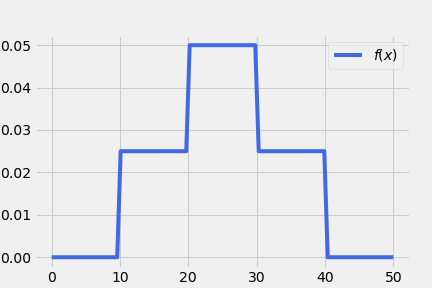
\includegraphics[scale=0.7]{images/p4_density.png}
        \caption{Función de densidad}
    \end{figure}
    \subsubsection*{b)}
    \begin{align*}
        P (x\geq 15) 
        &= \int_{15}^\infty f_X(x) dx \\
        &= \int_{15}^{20} 0.025dx + \int_{20}^{30} 0.050dx + \int_{30}^{40} 0.025dx \\
        &= 5 \cdot 0.025 + 10 \cdot 0.050 + 10 \cdot 0.025 \\
        &= 0.875
    \end{align*}
    así mismo se tiene:
    \begin{align*}
        P(20 \leq x \leq 30) = \int_{20}^{30} f_X(x)dx = 0.625 \\
        P(x < 30) = \int_{10}^{30} f_X(x)dx = 0.75 \\
        P(36 > x ) = \int_{36}^\infty f_X(x)dx = 0.1
    \end{align*}

    \subsubsection*{c)}
    Por definición:
    \begin{align*}
        E(X) 
        &= \int_{10}^{40} xf_X(x)dx \\
        &= \int_{10}^{20} x0.025dx + \int_{20}^{30} x0.050dx + \int_{30}^{40} x0.025dx \\
        &= 0.025(\tfrac{20^2}{2}-\tfrac{10^2}{2})+ 0.050(\tfrac{30^2}{2}-\tfrac{20^2}{2}) + 0.025(\tfrac{40^2}{2}-\tfrac{30^2}{2}) \\
        &= 25
    \end{align*}
    \begin{align*}
        var(X)
        &= E(X^2)-E(X)^2 \\
        &= \int_{10}^{40}x^2f_X(x)dx - (25)^2 \\
        &= \int_{10}^{20} x^2 0.025dx + \int_{20}^{30} x^2 0.050dx + \int_{30}^{40} x^2 0.025dx - (25)^2 \\
        &= 0.025(\tfrac{20^3}{3}-\tfrac{10^3}{3})+ 0.050(\tfrac{30^3}{3}-\tfrac{20^3}{3}) + 0.025(\tfrac{40^3}{3}-\tfrac{30^3}{3}) - (25)^2 \\
        &= 683.33 - (25)^2\\
        &= 58.33
    \end{align*}
\end{tcolorbox}

\section*{5.-}
\begin{enumerate}[a)]    
    \item Sea $X$ una variable aleatoria normal de parámetros $\mu$ y $\sigma^2$. Demostrar que la variable aleatoria $Y = aX+b$ con $a>0,b\in R$, 
    es una variable aleatoria normal de parámetros $a\mu +b$ y $a^2\sigma^2$.
    \item Sea $X$ una variable aleatoria Poisson con parámetro $\lambda$. Calcular la probabilidad de que $X$ tome sólo valores pares, i.e. $P(X es par)$.
\end{enumerate}
\begin{tcolorbox}[breakable]
    \subsubsection*{a)}
    Comenzamos con la relacion:
    \begin{align*}
        F_Y(y) 
        &= P(Y \leq y) \\
        &= P(aX+b \leq y) \\
        &= P(X \leq \tfrac{y-b}{a}) \\
        &= F_X(\tfrac{y-b}{a})
    \end{align*}
    obtenemos $f_Y(y)$ mediante la relación:
    \begin{align*}
        f_Y(y) 
        &= F_Y'(y) \\
        &= F_X'(\tfrac{y-b}{a})\tfrac{1}{a} \\
        &= f_X(\tfrac{y-b}{a})\tfrac{1}{a} \\
        &= \tfrac{1}{(a\sigma) \sqrt{2 \pi}}exp\left[{\tfrac{(y-(a\mu+b))^2}{2(a\sigma)^2}}\right] \\
    \end{align*}
    de donde podemos ver:
    \[ \mu_y = a\mu+b, \sigma_y = a^2\sigma^2 \]
    
    \subsubsection*{b)}
    La pmf para $X$ es:
    \[ p(n) = \frac{\lambda^ne^{-\lambda}}{n!}, \quad n \in N_0 \]
    Sumamos las probabilidad de todos los outcomes que favorecen este evento:
    \begin{align*}
        P(X par) 
        &= \sum_{n=0}^\infty p(2n) \\
        &= \sum_{n=0}^\infty \frac{\lambda^{2n}e^{-\lambda}}{(2n)!} \\
        &= e^{-\lambda}cosh(\lambda) \\
        &= \frac{1+e^{-2\lambda}}{2}
    \end{align*}
\end{tcolorbox}

\section*{6.-}
La cantidad de lluvia que cae en Ciudad de México anualmete es una variable aleatoria normal de media $840$ milímetros y desviación típica $150$ milímetros.
\begin{enumerate}[a)]
    \item ¿Cuál es la probabilidad de que en $2020$ llueva más de $900$ milímetros?
    \item ¿Cuál es la probabilidad de que en los próximos $7$ años haya exactamente $3$ años 
    donde se superen los $900$ milímetros?
\end{enumerate}
Expresar las probabilidades en términos de la función de distribución $\Phi(z)$ de la variable aleatoria 
normal estándar.
\begin{tcolorbox}[breakable]
    \subsubsection*{a)}
    Llamemos $Z$ a la variable aleatoria, usando la cdf de $Z$ tenemos:
    \begin{align*}
        P(Z \geq 900) 
        &= 1-F(900) \\
        &= 1-\Phi(\tfrac{900-840}{150}) \\
        &= 1-\Phi(\tfrac{2}{5})
    \end{align*} 
    \subsubsection*{b)}
    Llamemos $E$ al evento donde en exactamente 3 años se supera los $900$. \\
    Después de siete años se registra un outcomes de la forma:
    \[ Y|N,Y|N,...,Y|N \]
    donde por ejemplo el outcome $YYYNNNN$ nos dicé que los primeros 3 años se supero 
    los $900ml$ y los siguientes 4 años no, si llamamos a $p$ la probabildiad de que en un año llueva más de $900ml$
    se tiene:
    \begin{align*}
        P(E) &= C(7,3)p^3(1-p)^{7-3}, \quad p = 1-\Phi(\tfrac{2}{5})
    \end{align*}
\end{tcolorbox}

\section*{7.-}
Calcular el valor esperado $E(X)$ y la varianza $Var(X)$ de las siguientes variables aleatorias. Además, para cada una de ellas, mostrar una aplicación  
real en la cual se usen dichas variables aleatorias.

\begin{enumerate}[a)]
    \item $X$ es una variable aleatoria \textit{geométrica} con distribución de probabildiad:
    \[ P (X = n) = (1-p)^{n-1}p, \quad n = 1,2,...,0 \quad 0<p<1 \]
    \item $X$ es una variable aleatoria \textit{binominal negativa} con distribución de probabilidad:
    \[ P (X = n) =  \left( \begin{matrix} n-1 \\ r-1 \end{matrix} \right)p^r(1-p)^{n-r}, \quad n=r,r+1,..., \quad 0<p<1, \quad r\in N\]
    \item $X$ es una variable aleatoria con \textit{distribución Gamma} con función de densidad:
    \[ f(x) = \frac{\lambda e^{-\lambda x}(\lambda x)^{\alpha-1}}{\Gamma(\alpha)}, \quad \alpha,\lambda > 0, \quad x>0 \]
    donde $\Gamma(\alpha)$ es la función \textit{Gamma}.
    \item $X$ es una variable aleatoria con \textit{distribución Cauchy} con una función de densidad:
    \[ f(x) = \frac{1}{\pi} \frac{1}{1+x^2}, \quad x \in R \]
    \item $X$ es una variable aleatoria con \textit{distribución Beta} con una función de densidad:
    \[ f(x) = \frac{1}{B(a,b)}x^{a-1}(1-x)^{b-1}, \quad a,b>0, \quad 0<x<1 \]
    donde $B(a,b)$ es la función Beta.
\end{enumerate}
\begin{tcolorbox}[breakable]
    \subsection*{a)}
    \subsubsection*{Valor esperado}
    \begin{align*}
        E(X) 
        &= \sum_{x \in \Omega} xp(x) \\
        &= \sum_{n=1}^\infty n(1-p)^{n-1}p \\
        &= p\sum_{n=1}^\infty n(1-p)^{n-1} \\ 
        &= p(1+2(1-p)+3(1-p)^2+4(1-p)^3+...) \\
        &= p(\sum_{n=1}^\infty (1-p)^{n-1} + \sum_{n=2}^\infty (1-p)^{n-1} + ... \\
        &= p(\tfrac{1}{1-(1-p)} + \tfrac{1-p}{1-(1-p)} + \tfrac{(1-p)^2}{1-(1-p)} +... \\
        &= 1+(1-p)+(1-p)^2+... \\
        &= \frac{1}{1-(1-p)} \\
        &= \frac{1}{p} \\
    \end{align*}
    \subsubsection*{Varianza}
    \begin{align*}
        Var(X) 
        &= E(X^2)-E(X)^2 \\
        &= p\sum_{n=1}^\infty n^2(1-p)^{n-1} - \frac{1}{p^2} \\
        &= p\frac{1+(1-p)}{(1-(1-p))^3} - \frac{1}{p^2} \\
        &= \frac{2-p-1}{p^2} \\
        &= \frac{1-p}{p^2}
    \end{align*}
    \subsubsection*{Aplicación en la vida real}
    Supongamos que en una población el $20\%$ de las personas conocen primeros auxilios,
    queremos saber en promedio a cuántas personas se les debe preguntar 
    antes de encontrar una que sepa primeros auxilios. \\
    Llamemos $X$ a la variable aleatoria igual al número de personas que debemos preguntar
    \textbf{antes} de encontrar una que sepa primeros auxilios, entonces:
    \[ P(X=n) = (1-.2)^{n-1}.2 \]
    por ejemplo un outcome para este experimento es $NNY$, esto indica que preguntamos a tres personas, 
    las primeras dos no saben y la tercera sí. \\
    De acuerdo al valor promedio calculado se tiene:
    \[E(X) = \frac{1}{.2} = 5\]
    Esto es, en promedio se debe preguntar a $5$ personas antes de encontrar una que sepa primeros auxilios.
    \begin{figure}[H]
        \centering
        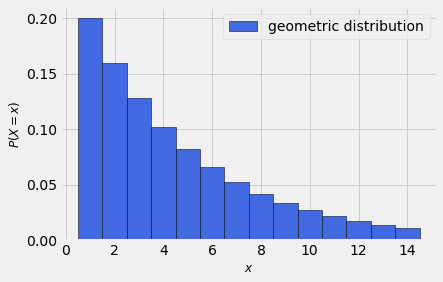
\includegraphics[scale=0.7]{images/p7_geometric.png}
        \caption{Distribución geométrica para $p=0.2$}
    \end{figure}
    \subsection*{b)}
    \subsubsection*{Valor esperado}
    \begin{align*}
        E(X) 
        &= \sum_{x \in \Omega} xp(x) \\
        &= \sum_{n=r}^\infty n\left( \begin{matrix} n-1 \\ r-1 \end{matrix} \right)p^r(1-p)^{n-r} \\
        &= \sum_{n=r}^\infty r\left( \begin{matrix} n \\ r \end{matrix} \right)p^r(1-p)^{n-r} \\  
        &= \frac{r}{p}\sum_{n=r+1}^\infty \left( \begin{matrix} n-1 \\ (r+1)-1 \end{matrix} \right)p^{r+1}(1-p)^{n-(r+1)} \\
        &= \frac{r}{p}
    \end{align*}
    ya que la última suma da 1 debido a que es la suma de todo el espacio de una variable con aleatoria dada por $NB(r+1,p)$.
    \subsubsection*{Varianza}
    \begin{align*}
        Var(X) 
        &= E(X^2)-E(X)^2 \\
        &= E(X(X+1))-E(X)-E(X)^2 \\
        &= \sum_{n=r}^\infty n(n+1)\left( \begin{matrix} n-1 \\ r-1 \end{matrix} \right)p^r(1-p)^{n-r}
        -\frac{rp}{p^2} - \frac{r^2}{p^2} \\
        &= r(r+1) \sum_{n=r}^\infty \left( \begin{matrix} n+1 \\ r+1 \end{matrix} \right)p^r(1-p)^{n-r} 
        -\frac{rp}{p^2} - \frac{r^2}{p^2} \\
        &= \frac{r(r+1)}{p^2} \sum_{n=r+2}^\infty \left( \begin{matrix} n-1 \\ (r+2)-1 \end{matrix} \right)p^{r+2}(1-p)^{n-(r+2)}
        -\frac{rp}{p^2} - \frac{r^2}{p^2} \\
        &= \frac{r^2+r}{p^2}-\frac{rp}{p^2} - \frac{r^2}{p^2} \\
        &= \frac{r(1-p)}{p^2}
    \end{align*}
    ya que la útlima suma infinita da 1 debido a que es la suma de todo el espacio de una variable con aleatoria dada por $NB(r+2,p)$.
    \subsubsection*{Aplicación en la vida real}
    Supongamos que se fábrican chips y cada uno tiene una probabilidad $p$ de fallar,
    nuestra variable aleatoria $X$ es el número de chips que debemos análisar \textbf{antes} de que 
    encontremos $r$ chips que fallan. \\
    Digamos $r=3,q=0.3$, un outcome para este problema es por ejemplo $WWWFFF$, donde quiere decir 
    que los primeros 3 chips que análisamos funcionan y los últimos $3$ no funcionan, se tiene entonces:
    \[ P (X = n) =  \left( \begin{matrix} n-1 \\ 3-1 \end{matrix} \right).3^3(1-.3)^{n-3}, \quad n=r,r+1,...\]
    \begin{figure}[H]
        \centering
        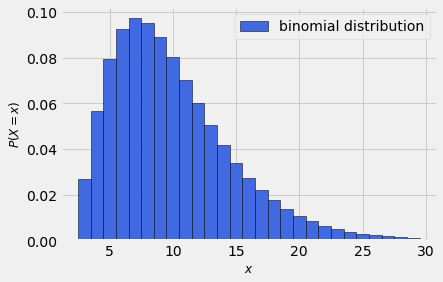
\includegraphics[scale=0.7]{images/p7_binomial.png}
        \caption{Distribución binominal negativa para $r=3,p=0.3$}
    \end{figure}
    \subsection*{c)} 
    \subsubsection*{Valor esperado}
    \begin{align*}
        E(X)
        &= \int_\Omega xf_X(x)dx \\
        &= \int_0^\infty xf_X(x)dx \\
        &= \int_0^\infty x\frac{\lambda e^{-\lambda x}(\lambda x)^{\alpha-1}}{\Gamma(\alpha)}dx \\
        &= \frac{\lambda^\alpha}{\Gamma(\alpha)} \int_0^\infty e^{-\lambda x}x^\alpha dx \\
        &= \frac{\lambda^\alpha}{\Gamma(\alpha)} \frac{\Gamma(\alpha+1)}{\lambda^{\alpha+1}} \\
        &= \frac{\alpha \Gamma(\alpha)}{\lambda \Gamma(\alpha)} \\
        &= \frac{\alpha}{\lambda} \\
    \end{align*}
    \subsubsection*{Varianza}
    \begin{align*}
        Var(X) &= E(X^2)-E(X)^2 \\
        &= \int_0^\infty x^2f_X(x)dx
        -\frac{\alpha^2}{\lambda^2} \\
        &= \frac{\lambda^\alpha}{\Gamma(\alpha)} \int_{0}^\infty x^{\alpha+1}e^{-\lambda x}dx
        -\frac{\alpha^2}{\lambda^2} \\
        &= \frac{\lambda^\alpha}{\Gamma(\alpha)} \frac{\Gamma(\alpha+2)}{\lambda^{\alpha+2}} 
        -\frac{\alpha^2}{\lambda^2} \\
        &= \frac{(\alpha+1)\Gamma(\alpha+1)}{\Gamma(\alpha)\lambda^2}
        -\frac{\alpha^2}{\lambda^2} \\
        &= \frac{(\alpha+1)\alpha \Gamma(\alpha)}{\lambda^2 \Gamma(\alpha)}
        -\frac{\alpha^2}{\lambda^2} \\
        &= \frac{\alpha(\alpha+1)}{\lambda^2} -\frac{\alpha^2}{\lambda^2} \\
        &= \frac{\alpha(\alpha+1)-\alpha}{\lambda^2} \\
        &= \frac{\alpha}{\lambda^2}
    \end{align*}
    \subsubsection*{Aplicación en la vida real}
    Supongamos que el tiempo de llegada de los clientes de un restaurante 
    esta modelado por un proceso de Poisson con un ratio $\lambda=1$, esto es un cliente por unidad de tiempo,
    llamamos $X$ a la variable aleatoria que nos dice la hora de llegada del $5$to cliente, entonces: 
    \[ X \sim Gamma(5,1) \]
    \begin{figure}[H]
        \centering
        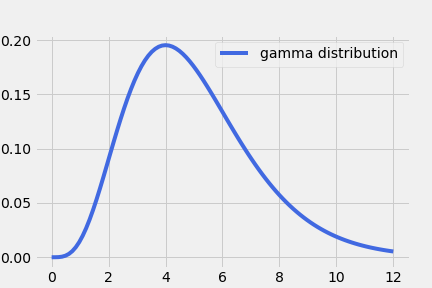
\includegraphics[scale=0.7]{images/p7_gamma.png}
        \caption{Distribución Gamma con $\alpha=5, \lambda=1$}
    \end{figure}
    \subsection*{d)}
    \subsubsection*{Valor esperado}
    \begin{align*}
        E(X) 
        &= \int_\Omega xf_X(x)dx \\
        &= \int_{-\infty}^\infty xf_X(x)dx \\
        &= \int_{-\infty}^\infty \frac{1}{\pi}\frac{x}{1+x^2}dx \\ 
        &= \frac{1}{2\pi}ln(1+x^2)\bigg|_{-\infty}^\infty \\
        &= 0 \\
    \end{align*}
    \subsubsection*{Varianza}
    \begin{align*}
        Var(X)&= E(X^2)-E(X)^2 \\
        &= \int_{-\infty}^\infty x^2f_X(x)dx \\
        &= \int_{-\infty}^\infty \frac{1}{\pi}\frac{x^2}{1+x^2}dx \\
        &= \frac{x-arctan(x)}{\pi} \bigg|_{-\infty}^\infty \\
        &= undefined
    \end{align*}
    \subsubsection*{Aplicación en la vida real}
    Supongamos que queremos estudiar el movimiento de un tiburón en busca de comida
    cuando este es colocado en un área aleatoria del océano, veremos que en general sigue el 
    movimiento Browniano, pero en ausencia de comida el movimiento que sigue es el \textit{Levy flight}, 
    donde la dirección angular esta dada por una distribución normal y el tamaño del paso por una distribución de Cauchy,
    esto es si llamamos a $X$ la variable aleatoria que nos dice el tamaño de paso que se realiza en cada movimiento, se tiene:
    \[X \sim Cauchy \]
    \begin{figure}[H]
        \centering
        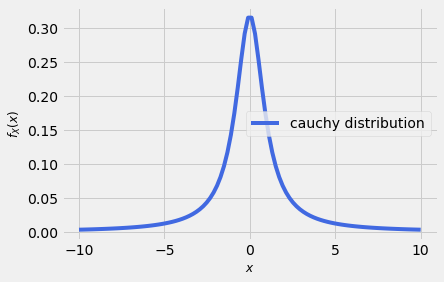
\includegraphics[scale=0.7]{images/p7_cauchy.png}
        \caption{Distribución Cauchy}
    \end{figure}
    \subsection*{e)}
    \subsubsection*{Valor esperado}
    \begin{align*}
        E(X)
        &= \int_\Omega xf_X(x)dx \\
        &= \int_{0}^1 xf_X(x)dx \\
        &= \frac{1}{B(\alpha,\beta)} \int_{0}^1 x^\alpha(1-x)^{\beta-1}dx \\
        &= \frac{B(\alpha+1,\beta)}{B(\alpha,\beta)} \\
        &= \frac{\Gamma(\alpha+1)\Gamma(\beta)}{\Gamma(\alpha+\beta+1)} \cdot \frac{\Gamma(\alpha + \beta)}{\Gamma(\alpha)\Gamma(\beta)} \\
        &= \frac{\alpha}{\alpha + \beta} \frac{\Gamma(\alpha) \Gamma(\beta) \Gamma(\alpha + \beta)}{\Gamma(\alpha) \Gamma(\beta) \Gamma(\alpha + \beta)} \\
        &= \frac{\alpha}{\alpha + \beta} \\
    \end{align*}
    \subsubsection*{Varianza}
    \begin{align*}
        Var(X)&= E(X^2)-E(X)^2 \\
        &= \int_{0}^1 x^2f_X(x)dx 
        - \frac{\alpha^2}{(\alpha+\beta)^2} \\
        &= \frac{B(\alpha+2,\beta)}{B(\alpha, \beta)} 
        - \frac{\alpha^2}{(\alpha+\beta)^2} \\
        &= \frac{\Gamma(\alpha+2)\Gamma(\beta)}{\Gamma(\alpha+\beta+2)} \frac{\Gamma(\alpha+\beta)}{\Gamma(\alpha)\Gamma(\beta)}
        - \frac{\alpha^2}{(\alpha+\beta)^2} \\
        &= \frac{\alpha(\alpha+1)}{(\alpha+\beta)(\alpha+\beta+1)} \frac{\Gamma(\alpha)\Gamma(\beta)\Gamma(\alpha+\beta)}{\Gamma(\alpha)\Gamma(\beta)\Gamma(\alpha+\beta)} 
        - \frac{\alpha^2}{(\alpha+\beta)^2} \\
        &= \frac{\alpha(\alpha+1)(\alpha+\beta)}{(\alpha+\beta)^2(\alpha+\beta+1)} - \frac{\alpha^2(\alpha+\beta+1)}{(\alpha+\beta)^2(\alpha+\beta+1)} \\
        &= \frac{\alpha^3+\alpha^2\beta+ \alpha^2+\alpha \beta-\alpha^3- \alpha^2\beta  - \alpha^2}{(\alpha+\beta)^2(\alpha+\beta+1)} \\
        &= \frac{\alpha \beta}{(\alpha+\beta)^2(\alpha+\beta+1)}
    \end{align*}
    \subsubsection*{Aplicación en la vida real}
    Supongamos que estamos comprando en amazon y vemos dos vendedores para el mismo producto:
    \begin{itemize}
        \item Vendedor A $94\%$ reviews positivas de $80$
        \item Vendedor B $100\%$ reviews positivas de $8$
    \end{itemize}
    Llamemos $p$ a la variable aleatoria que nos dice la probabildiad de que para un 
    determinado vendedor un comprador de una review positiva. \\
    Nuestro prior para $p$ es una distribución $\pi=Beta$, por ejemplo si 
    no hay reviews del vendedor entonces:
    \[ p \sim Beta(1,1) = U(0,1) \]
    ahora bien, sabiendo que hay $x$ número de reviews positivas de un total de $n$ reviews, 
    actualizamos la distribución para $p$ de la siguiente manera:
    \begin{align*}
        \pi(p|x) 
        &= C \pi(p) f(x|p) \\
        &= Beta(\alpha+x,n-x+\beta)
    \end{align*}
    en nuestro caso después de actualizar tenemos:
    \[ p_A \sim Beta(76,6), \quad p_B \sim Beta(9,1) \]
    \begin{figure}[H]
        \centering
        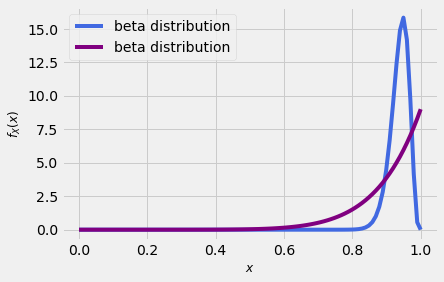
\includegraphics[scale=0.7]{images/p7_beta.png}
        \caption{Distribución Beta para $p_A$(azul) y $p_B$(morado)}
    \end{figure}
    donde podemos ver:
    \[ P(p_a > 0.85) > P(p_b > 0.85) \]
    el cuál podria ser un buen criterio para elegir a $A$ sobre $B$

\end{tcolorbox}



\end{document}
